\documentclass[11pt]{article}
\usepackage[margin=1in]{geometry}
\usepackage{amsmath,amssymb}
\usepackage{lmodern}
\usepackage[T1]{fontenc}
\usepackage{enumitem}
\usepackage{microtype}
\usepackage{tikz}
\usetikzlibrary{arrows.meta,angles,quotes,calc,decorations.pathreplacing}

\title{2016 F=ma Exam Review}
\author{Nathan P.}
\date{January 1, 2026}

\begin{document}
\maketitle

\section*{Problem 1}
A concise way of thinking:
\[
\frac{\omega_L}{\omega_R}=\frac{\text{circle}_L/\text{time}}{\text{circle}_R/\text{time}}=\frac{2\pi R}{2\pi(R+1.74)}.
\]
$\omega$ around the curve is the same for both, so $v/r$ is the same for both, so
\[
\frac{r\,\omega_{\text{left}}}{R}=\frac{r\,\omega_{\text{right}}}{R+1.74},
\]
then you can find the ratio of $\omega_{\text{left}}$ to $\omega_{\text{right}}$.

\section*{Problem 3}
Energy conservation is best and concise: $E_i+W_{\text{ext}}=E_f$.
Or use kinematics, and don't forget to \emph{sum} the forces. The force up \emph{also} has to overcome $mg$ to accelerate it up.

\section*{Problem 4}
There's tangential and centripetal acceleration; the question is whether $a_c$ increases linearly or nonlinearly.
$a_c=v^2/r$ and $v$ depends on a constant forward acceleration times $t$, so $v^2$ depends on $t^2$, so the total acceleration is
\[
a=\sqrt{(g\sin\theta)^2+a_c^2}=\sqrt{(g\sin\theta)^2+Ct^4},
\]
where $C$ is some constant. $\sqrt{Ct^4}$ isn't linear.
Learn to simplify expressions about general relationships by subbing in constants.

\section*{Problem 8}
Conservation of angular momentum is independent of the nature of the central force. While it depends on $r$, it doesn't depend on the force, because a central force goes through the axis of rotation, providing no torque, meaning $\Delta L$ still $=0$.

\section*{Problem 9}
``Frictionless'' $\to$ use energy conservation. The glass sphere does no work because it doesn't have any displacement and the normal force is always perpendicular to the bead's motion.
Use circular motion:
\[
mg\cos\theta-N=\frac{mv^2}{R}.
\]
$N=0$ when it loses contact.
Some mathematical conveniences: $R=D/2$ (sub it in later). $h=R(1-\cos\theta)$, you've seen that.

\begin{center}
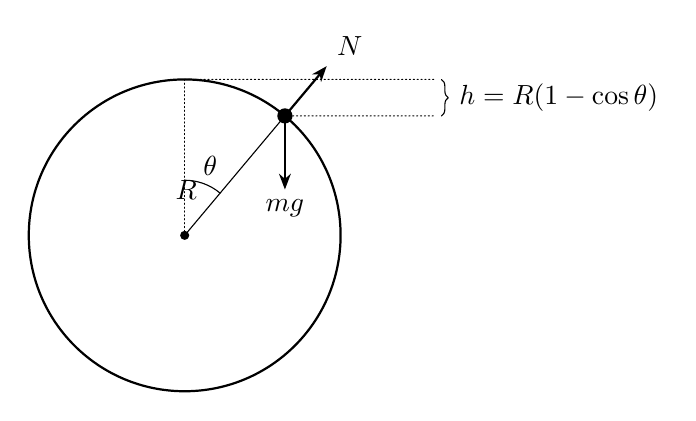
\begin{tikzpicture}[scale=1.1, line cap=round, line join=round, >={Stealth[length=2mm]}]
  \coordinate (O) at (0,0);
  \coordinate (T) at (0,1.8);
  \coordinate (B) at (50:1.8);
  \draw[thick] (O) circle (1.8);
  \fill (O) circle (1.5pt);
  \draw[densely dotted] (O) -- (T);
  \draw (O) -- (B) node[pos=0.22, above left] {$R$};
  \pic[draw, "$\theta$", angle radius=7mm, angle eccentricity=1.35] {angle = B--O--T};
  \fill (B) circle (2.5pt);
  \draw[->,thick] (B) -- ++(0,-0.85) node[below] {$mg$};
  \draw[->,thick] (B) -- ++(50:0.75) node[above right] {$N$};
  \draw[densely dotted] (T) -- (2.9,1.8);
  \draw[densely dotted] (B) -- (2.9,{1.8*sin(50)});
  \draw[decorate, decoration={brace, raise=2pt}] (2.9,1.8) -- (2.9,{1.8*sin(50)})
    node[midway, right=5pt] {$h=R(1-\cos\theta)$};
\end{tikzpicture}
\end{center}

\section*{Problem 10}
For tension $T_2$ to change, the string must change its length, and it can't do so because at that instant $m_1$ hasn't moved.

\section*{Problem 11}
Write out what's given: $P\propto m$.
The answer is in terms of $v$ and $m$, so get rid of everything else by recognizing the relationship between $m$ and $A$.

\section*{Problem 14}
Use the $\ddot{x}=-\omega^2x$ concept.

\section*{Problem 15}
$\sin\theta\approx\theta$, use the same SHM concept.
See that it's the same restoring force applied at the same distance $\to$ same frequency/period.

\section*{Problem 19}
Write out equations with $H$, $R$, $D$, and relate them by plugging in.
Energy is conserved, especially in these situations where something slides frictionlessly on a surface that doesn't move and exerts only an orthogonal force ($W=0$).

\section*{Problem 20}
No slipping condition: $\mu=\tan\theta$.
When it reaches the angle where $mg$ passes through the pivot point, it should have $\mu\ge\tan\theta$.
$\theta$ can be found via triangle geometry (vertex to com : com to side midpoint $=2:1$).

\begin{center}
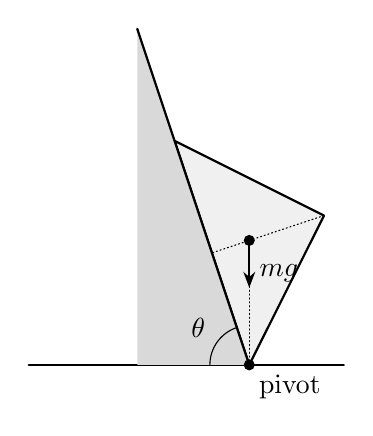
\begin{tikzpicture}[scale=1.0, line cap=round, line join=round, >={Stealth[length=2mm]}]
  % right-isosceles prism (w = 2h) at the critical angle: mg passes through the downhill corner P
  \coordinate (Z) at (0,0);
  \coordinate (P) at (2.2,0);
  \draw[thick] (-0.6,0) -- (3.4,0);
  \begin{scope}[scale=1.5, rotate around={-71.57:(P)}]
    \coordinate (Q) at ($(P)+(-2,0)$);
    \coordinate (V) at ($(P)+(-1,1)$);
    \coordinate (Mid) at ($(P)+(-1,0)$);
    \coordinate (G) at ($(P)+(-1,0.3333)$);
    \coordinate (Top) at ($(P)+(-3.0,0)$);
    \draw[thick, fill=gray!12] (P) -- (Q) -- (V) -- cycle;
    \draw[densely dotted] (V) -- (Mid);
  \end{scope}
  \fill[gray!30] (P) -- (Top) -- (Top |- P) -- cycle;
  \draw[thick] (P) -- (Top);
  \draw[densely dotted] (P) -- ++(0,1.6);
  \fill (G) circle (2pt);
  \draw[->,thick] (G) -- ++(0,-0.6) node[pos=0.7,right] {$mg$};
  \fill (P) circle (2pt) node[below right] {pivot};
  \pic[draw, "$\theta$", angle radius=5mm, angle eccentricity=1.6] {angle = Top--P--Z};
\end{tikzpicture}
\end{center}

\section*{Problem 22}
Energy (and horizontal momentum) of the system is conserved! The normal force from the ground does no work.
Fact: a force does work only if the point of application moves in the direction of the force.
Neither ball has horizontal velocity at the end (horizontal momentum is conserved and $=0$).
All the initial potential of the system gets transferred to kinetic, and the KE is concentrated in the top ball because the bottom ball has $v=0$ and the rod is massless.
The bottom ball cannot have $v_x$, otherwise the top mass must have the same $v_x$ (they're horizontal, incompressible rod), but that would violate momentum conservation.

\section*{Review}

\subsection*{Problem 6}
Fact: uniformly accelerated motion is just parabolic.

\subsection*{Problem 17}
$0$ torque about the IAOR (instantaneous axis of rotation), or contact point with the ground, so $\Delta L=0$:
\[
mvR+I\omega=0,\qquad mvR=-\tfrac23 mR^2\omega,\qquad |v|=\tfrac23 R\omega.
\]

\subsection*{Problem 25}
Uncertain quantities added together have errors adding in quadrature.
\begin{itemize}[leftmargin=*, itemsep=0.25em]
\item A: $2$
\item B: $\sqrt{2^2+2^2}=\sqrt{8}=2\sqrt{2}$
\item C: $\sqrt{2}$
\end{itemize}

\end{document}
